%!TEX root = ../Thesis.tex
\chapter{Stochastic Bilinear Model with Chance Constraints}

\section{Stochastic Bilinear System}
\label{sec:stochastic_bilinear_system}

A stochastic bilinear system is considered in the form

\begin{align}
    x_{k+1}
    &=
    A(v_k)x_k
    +
    B(v_k)u_k
    +
    w_k
    \label{eq:sb_state}\\
    y_k
    &=
    Cx_k+\eta_k
    \label{eq:sb_output}
\end{align}

where \(u_k\) denotes the control input and \(v_k\) is the
bilinear scheduling variable. The stochastic disturbances are assumed to be
zero-mean Gaussian,

\begin{align}
    w_k &\sim \mathcal{N}(0,R_w)\\
    \eta_k &\sim \mathcal{N}(0,R_\eta)
\end{align}

and the initial state is distributed according to

\begin{equation}
    x_0 \sim \mathcal{N}(\mu_0,P_0)
\end{equation}

For compactness, the time-varying system matrices are denoted by

\begin{equation}
    A_k=A(v_k),
    \qquad
    B_k=B(v_k)
\end{equation}

\subsection{System Matrices}

The state distribution at time step \(k\) is characterized by its mean
and covariance,

\begin{equation}
    x_k \sim \mathcal{N}(\mu_k,P_k)
\end{equation}

The state mean is defined as

\begin{equation}
    \mu_k=\mathbb{E}[x_k]
\end{equation}

Taking the expectation of \cref{eq:sb_state} gives

\begin{align}
    \mu_{k+1}
    &=
    \mathbb{E}
    \left[
        A_kx_k+B_ku_k+w_k
    \right] \\
    &=
    A_k\mathbb{E}[x_k]
    +
    B_ku_k
    +
    \mathbb{E}[w_k]
\end{align}

Since the process noise is zero mean,

\begin{equation}
    \boxed{
    \mu_{k+1}
    =
    A_k\mu_k+B_ku_k
    }
    \label{eq:sb_mean}
\end{equation}

To derive the covariance, the state is decomposed as

\begin{equation}
    x_k=\mu_k+e_k,
\end{equation}

where

\begin{equation}
    e_k=x_k-\mu_k,
    \qquad
    \mathbb{E}[e_k]=0
\end{equation}

Using the state and mean equations,

\begin{align}
    x_{k+1}
    &=
    A_k\mu_k+B_ku_k+A_ke_k+w_k\\
    \mu_{k+1}
    &=
    A_k\mu_k+B_ku_k
\end{align}

and therefore

\begin{equation}
    e_{k+1}
    =
    A_ke_k+w_k
\end{equation}

The state covariance is

\begin{equation}
    P_{k+1}
    =
    \mathbb{E}
    \left[
        e_{k+1}e_{k+1}^T
    \right]
\end{equation}

Substituting the error dynamics gives

\begin{align}
    P_{k+1}
    &=
    \mathbb{E}
    \left[
        (A_ke_k+w_k)
        (A_ke_k+w_k)^T
    \right]\\
    &=
    A_kP_kA_k^T
    +
    A_k\mathbb{E}[e_kw_k^T]
    +
    \mathbb{E}[w_ke_k^T]A_k^T
    +
    R_w
\end{align}

Assuming that the process noise is independent of the state error, the
cross terms vanish, giving

\begin{equation}
    \boxed{
    P_{k+1}
    =
    A_kP_kA_k^T+R_w
    }
    \label{eq:sb_covariance}
\end{equation}

Since \(A_k=A(v_k)\), the propagated covariance depends on the sequence
\(V\). Hence,

\begin{equation}
    P_k=P_k(V)
\end{equation}

The output mean follows from

\begin{equation}
    y_k=Cx_k+\eta_k
\end{equation}

Taking the expectation gives

\begin{equation}
    \boxed{
    \mu_{y,k}
    =
    \mathbb{E}[y_k]
    =
    C\mu_k
    }
    \label{eq:sb_output_mean}
\end{equation}

The corresponding output covariance is

\begin{equation}
    \boxed{
    P_{y,k}
    =
    CP_kC^T+R_\eta
    }
    \label{eq:sb_output_covariance}
\end{equation}

Since \(P_k=P_k(V)\),

\begin{equation}
    P_{y,k}=P_{y,k}(V)
\end{equation}

\subsection{Stacked Matrix Derivations}

The first predicted state mean is

\begin{equation}
    \mu_1=A_0\mu_0+B_0u_0.
\end{equation}

The second predicted mean becomes

\begin{align}
    \mu_2
    &=
    A_1\mu_1+B_1u_1\\
    &=
    A_1A_0\mu_0
    +
    A_1B_0u_0
    +
    B_1u_1
\end{align}

Similarly,

\begin{equation}
    \mu_3
    =
    A_2A_1A_0\mu_0
    +
    A_2A_1B_0u_0
    +
    A_2B_1u_1
    +
    B_2u_2
\end{equation}

In general,

\begin{equation}
    \mu_k
    =
    A_{k-1}\cdots A_0\mu_0
    +
    \sum_{j=0}^{k-1}
    A_{k-1}\cdots A_{j+1}B_ju_j
\end{equation}

where an empty matrix product is interpreted as the identity matrix.

Define the stacked vectors

\begin{equation}
    M=
    \begin{bmatrix}
        \mu_1\\
        \mu_2\\
        \vdots\\
        \mu_N
    \end{bmatrix},
    \qquad
    U=
    \begin{bmatrix}
        u_0\\
        u_1\\
        \vdots\\
        u_{N-1}
    \end{bmatrix},
    \qquad
    V=
    \begin{bmatrix}
        v_0\\
        v_1\\
        \vdots\\
        v_{N-1}
    \end{bmatrix}
\end{equation}

The stacked state-mean prediction becomes

\begin{equation}
    \boxed{
    M
    =
    \mathcal{A}(V)\mu_0
    +
    \mathcal{B}(V)U
    }
\end{equation}

The matrix \(\mathcal{A}(V)\) is

\begin{equation}
    \mathcal{A}(V)
    =
    \begin{bmatrix}
        A_0\\
        A_1A_0\\
        A_2A_1A_0\\
        \vdots\\
        A_{N-1}A_{N-2}\cdots A_0
    \end{bmatrix}
\end{equation}

while

\begin{equation}
\mathcal{B}(V)
=
\begin{bmatrix}
B_0 & 0 & \cdots & 0\\
A_1B_0 & B_1 & \cdots & 0\\
A_2A_1B_0 & A_2B_1 & \cdots & 0\\
\vdots & \vdots & \ddots & \vdots\\
A_{N-1}\cdots A_1B_0 &
A_{N-1}\cdots A_2B_1 &
\cdots &
B_{N-1}
\end{bmatrix}
\end{equation}

For the outputs, define

\begin{equation}
    \mathcal{C}=I_N\otimes C.
\end{equation}

The stacked output-mean vector is

\begin{equation}
    M_y
    =
    \begin{bmatrix}
        \mu_{y,1}\\
        \mu_{y,2}\\
        \vdots\\
        \mu_{y,N}
    \end{bmatrix}
    =
    \mathcal{C}M
\end{equation}

Therefore,

\begin{equation}
    M_y
    =
    \mathcal{C}\mathcal{A}(V)\mu_0
    +
    \mathcal{C}\mathcal{B}(V)U
\end{equation}

Defining

\begin{equation}
    \Phi(V)
    =
    \mathcal{C}\mathcal{A}(V),
    \qquad
    \Gamma(V)
    =
    \mathcal{C}\mathcal{B}(V)
\end{equation}

gives

\begin{equation}
    \boxed{
    M_y
    =
    \Phi(V)\mu_0
    +
    \Gamma(V)U
    }
    \label{eq:sb_stacked_output}
\end{equation}

\section{Model with Chance Constraints}
\label{sec:sb_chance_constraints}

The probabilistic output constraint is

\begin{equation}
    \mathbb{P}
    \left(
        y_{\min}
        \leq
        y_k
        \leq
        y_{\max}
    \right)
    \geq
    1-\alpha
\end{equation}

The violation probability is divided as

\begin{equation}
    \alpha_{\mathrm{lower}}
    +
    \alpha_{\mathrm{upper}}
    =
    \alpha
\end{equation}

For the stochastic bilinear system,

\begin{equation}
    \mu_{y,k}
    =
    C\mu_k(U,V)
\end{equation}

while

\begin{equation}
    P_{y,k}(V)
    =
    CP_k(V)C^T+R_\eta
\end{equation}

For a scalar output, the corresponding standard deviation is

\begin{equation}
    \sigma_{y,k}(V)
    =
    \sqrt{
        CP_k(V)C^T+R_\eta
    }
\end{equation}

The upper chance constraint becomes

\begin{equation}
    C\mu_k(U,V)
    \leq
    y_{\max}
    -
    \Phi_{\mathcal{N}}^{-1}
    \left(
        1-\alpha_{\mathrm{upper}}
    \right)
    \sigma_{y,k}(V)
\end{equation}

while the lower constraint becomes

\begin{equation}
    C\mu_k(U,V)
    \geq
    y_{\min}
    +
    \Phi_{\mathcal{N}}^{-1}
    \left(
        1-\alpha_{\mathrm{lower}}
    \right)
    \sigma_{y,k}(V)
\end{equation}

where \(\Phi_{\mathcal{N}}^{-1}\) denotes the inverse CDF of the
standard normal distribution.

The tight bounds are therefore defined as

\begin{equation}
    \boxed{
    \tilde{y}_{\min,k}(V)
    =
    y_{\min}
    +
    \Phi_{\mathcal{N}}^{-1}
    (1-\alpha_{\mathrm{lower}})
    \sigma_{y,k}(V)
    }
\end{equation}

and

\begin{equation}
    \boxed{
    \tilde{y}_{\max,k}(V)
    =
    y_{\max}
    -
    \Phi_{\mathcal{N}}^{-1}
    (1-\alpha_{\mathrm{upper}})
    \sigma_{y,k}(V)
    }
\end{equation}

Hence,

\begin{equation}
    \boxed{
    \tilde{y}_{\min,k}(V)
    \leq
    C\mu_k(U,V)
    \leq
    \tilde{y}_{\max,k}(V)
    }
\end{equation}

Define

\begin{equation}
    \tilde{Y}_{\min}(V)
    =
    \begin{bmatrix}
        \tilde{y}_{\min,1}(V)\\
        \vdots\\
        \tilde{y}_{\min,N}(V)
    \end{bmatrix}
\end{equation}

and

\begin{equation}
    \tilde{Y}_{\max}(V)
    =
    \begin{bmatrix}
        \tilde{y}_{\max,1}(V)\\
        \vdots\\
        \tilde{y}_{\max,N}(V)
    \end{bmatrix}
\end{equation}

Using the stacked output-mean prediction,

\begin{equation}
    \boxed{
    \tilde{Y}_{\min}(V)
    \leq
    \Phi(V)\mu_0+\Gamma(V)U
    \leq
    \tilde{Y}_{\max}(V)
    }
    \label{eq:sb_stacked_chance}
\end{equation}

\section{Cost Function Derivation}
\label{sec:sb_cost}

The expected stochastic objective is defined as

\begin{equation}
    \phi
    =
    \frac{1}{2}
    \mathbb{E}
    \left[
        (Y-\bar{Y}_{\mathrm{ref}})^T
        Q
        (Y-\bar{Y}_{\mathrm{ref}})
        +
        U^TR_UU
        +
        V^TR_VV
    \right]
\end{equation}

Since \(U\) and \(V\) are deterministic optimization variables,

\begin{align}
    \phi
    &=
    \frac{1}{2}
    \mathbb{E}
    \left[
        (Y-\bar{Y}_{\mathrm{ref}})^T
        Q
        (Y-\bar{Y}_{\mathrm{ref}})
    \right]
    \nonumber\\
    &\quad+
    \frac{1}{2}U^TR_UU
    +
    \frac{1}{2}V^TR_VV
\end{align}

The stochastic output is decomposed as

\begin{equation}
    Y=M_y+E_y
\end{equation}

where

\begin{equation}
    \mathbb{E}[E_y]=0
\end{equation}

Substitution gives

\begin{align}
&\mathbb{E}
\left[
(Y-\bar{Y}_{\mathrm{ref}})^T
Q
(Y-\bar{Y}_{\mathrm{ref}})
\right]
\\
&=
(M_y-\bar{Y}_{\mathrm{ref}})^T
Q
(M_y-\bar{Y}_{\mathrm{ref}})
+
\mathbb{E}[E_y^TQE_y]
\end{align}

Using the trace identity,

\begin{equation}
    \mathbb{E}[E_y^TQE_y]
    =
    \operatorname{tr}
    \left(
        QP_Y
    \right)
\end{equation}

Therefore,

\begin{equation}
    \phi
    =
    \frac{1}{2}
    \left[
        (M_y-\bar{Y}_{\mathrm{ref}})^T
        Q
        (M_y-\bar{Y}_{\mathrm{ref}})
        +
        \operatorname{tr}(QP_Y)
        +
        U^TR_UU
        +
        V^TR_VV
    \right]
\end{equation}

For the stochastic bilinear model,

\begin{equation}
    M_y
    =
    \Phi(V)\mu_0+\Gamma(V)U
\end{equation}

and the output covariance also depends on \(V\). Hence,

\begin{equation}
\boxed{
\begin{aligned}
    \phi(U,V)
    =
    \frac{1}{2}
    \Big[
    &
    \left(
        \Phi(V)\mu_0
        +
        \Gamma(V)U
        -
        \bar{Y}_{\mathrm{ref}}
    \right)^T
    Q
    \left(
        \Phi(V)\mu_0
        +
        \Gamma(V)U
        -
        \bar{Y}_{\mathrm{ref}}
    \right)
    \\
    &+
    U^TR_UU
    +
    V^TR_VV
    +
    \operatorname{tr}
    \left(
        QP_Y(V)
    \right)
    \Big]
\end{aligned}
}
\label{eq:sb_cost_final}
\end{equation}

\section{Problem Overview}
\label{sec:sb_problem_overview}

Combining the stochastic bilinear cost function and the chance constraints
gives the complete optimization problem

\begin{equation}
\boxed{
\begin{aligned}
    \min_{U,V}
    \quad &
    \phi(U,V)
    \\[1mm]
    \text{subject to}
    \quad &
    \tilde{Y}_{\min}(V)
    \leq
    \Phi(V)\mu_0+\Gamma(V)U
    \leq
    \tilde{Y}_{\max}(V),
    \\
    &
    U_{\min}
    \leq U \leq
    U_{\max},
    \\
    &
    V_{\min}
    \leq V \leq
    V_{\max}
\end{aligned}
}
\label{eq:sb_final_problem}
\end{equation}

The decision vector can equivalently be written as

\begin{equation}
    z=
    \begin{bmatrix}
        U\\
        V
    \end{bmatrix}
\end{equation}


\section{Open-Loop Implementation}
\label{sec:sb_open_loop}

The stochastic bilinear open-loop implementation is evaluated using Monte
Carlo simulation. A single pair of optimal sequences \(U^\ast\) and \(V^\ast\)
is first obtained by solving the nonlinear optimization problem using SLSQP.

The optimization is performed only once:

\begin{equation}
    (U^\ast,V^\ast)
    =
    \arg\min_{U,V}\phi(U,V)
\end{equation}

subject to the chance constraints and the bounds on \(U\) and \(V\).

After the optimal sequences have been obtained, the same \(U^\ast\) and
\(V^\ast\) are applied to every Monte Carlo realization.

For realization \(j\),

\begin{equation}
    x_0^{(j)}
    \sim
    \mathcal{N}(\mu_0,P_0)
\end{equation}

and independent stochastic disturbances are sampled as

\begin{align}
    w_k^{(j)}
    &\sim
    \mathcal{N}(0,R_w)\\
    \eta_k^{(j)}
    &\sim
    \mathcal{N}(0,R_\eta)
\end{align}

All trajectories use

\begin{equation}
    u_k^{(j)}=u_k^\ast,
    \qquad
    v_k^{(j)}=v_k^\ast
\end{equation}

The stochastic dynamics are then simulated according to

\begin{equation}
    x_{k+1}^{(j)}
    =
    A(v_k^\ast)x_k^{(j)}
    +
    B(v_k^\ast)u_k^\ast
    +
    w_k^{(j)}
\end{equation}

and

\begin{equation}
    y_k^{(j)}
    =
    Cx_k^{(j)}
    +
    \eta_k^{(j)}
\end{equation}

Thus, the optimizer determines one common open-loop pair
\((U^\ast,V^\ast)\), while the Monte Carlo trajectories differ because of
their independently sampled initial conditions and stochastic disturbances.

\begin{enumerate}
    \item Define \(N\), \(\mu_0\), \(P_0\), \(Q\), \(R_U\), \(R_V\),
    \(R_w\), \(R_\eta\), the reference trajectory, chance-constraint
    parameters, and bounds on \(U\) and \(V\).

    \item Initialize candidate sequences \(U\) and \(V\).

    \item For each candidate \(V\), construct \(A_k\), \(B_k\),
    \(\Phi(V)\), \(\Gamma(V)\), and propagate \(P_k(V)\).

    \item Construct the \(V\)-dependent tight bounds.

    \item Evaluate the cost function \(\phi(U,V)\).

    \item Solve the constrained nonlinear problem using SLSQP to obtain
    \(U^\ast\) and \(V^\ast\).

    \item Generate the Monte Carlo realizations.

    \item Apply the same \(U^\ast\) and \(V^\ast\) to every realization.

    \item Evaluate the output trajectories and empirical constraint
    satisfaction.
\end{enumerate}

\subsection{Results}
\label{subsec:sb_open_loop_results}

The stochastic bilinear open-loop controller was evaluated over a horizon

\begin{equation}
    N=30.
\end{equation}

The bilinear state-transition matrix was defined as

\begin{equation}
    A(v)
    =
    A_{\mathrm{base}}
    +
    vA_v
\end{equation}

where

\begin{equation}
    A_{\mathrm{base}}
    =
    \begin{bmatrix}
        0.90 & 0\\
        0 & 0.50
    \end{bmatrix},
    \qquad
    A_v
    =
    \begin{bmatrix}
        0 & 1\\
        0 & 0
    \end{bmatrix}
\end{equation}

Hence,

\begin{equation}
    A(v)
    =
    \begin{bmatrix}
        0.90 & v\\
        0 & 0.50
    \end{bmatrix}
\end{equation}

The input matrix was

\begin{equation}
    B(v)
    =
    \begin{bmatrix}
        0\\
        1
    \end{bmatrix}
\end{equation}

and both states were directly observed,

\begin{equation}
    C=I_2
\end{equation}

The weighting matrices were

\begin{equation}
    Q=I_2,
    \qquad
    R_U=0.1,
    \qquad
    R_V=0.1
\end{equation}

The process and measurement noise covariance matrices were

\begin{equation}
    R_w
    =
    R_\eta
    =
    \begin{bmatrix}
        0.005 & 0\\
        0 & 0.005
    \end{bmatrix}
\end{equation}

The initial state distribution was

\begin{equation}
    \mu_0=
    \begin{bmatrix}
        0\\
        0
    \end{bmatrix},
    \qquad
    P_0=
    \begin{bmatrix}
        0.01 & 0\\
        0 & 0.01
    \end{bmatrix}
\end{equation}

The output bounds were

\begin{equation}
    y_{\min}
    =
    \begin{bmatrix}
        -1.7\\
        -1.7
    \end{bmatrix},
    \qquad
    y_{\max}
    =
    \begin{bmatrix}
        3.5\\
        3.5
    \end{bmatrix}
\end{equation}

with

\begin{equation}
    \alpha_{\mathrm{lower}}
    =
    \alpha_{\mathrm{upper}}
    =
    0.01
\end{equation}

The reference trajectory was

\begin{equation}
    \bar{y}_k
    =
    \begin{cases}
        [\,3.1\;\;-1.3\,]^T,
        & k=1,\ldots,15,\\[1mm]
        [\,-1.3\;\;3.1\,]^T,
        & k=16,\ldots,30
    \end{cases}
\end{equation}

The optimization variables were bounded by

\begin{align}
    -5 &\leq u_k \leq 5,\\
    -5 &\leq v_k \leq 5
\end{align}
\clearpage

\begin{figure}[H]
    \centering
    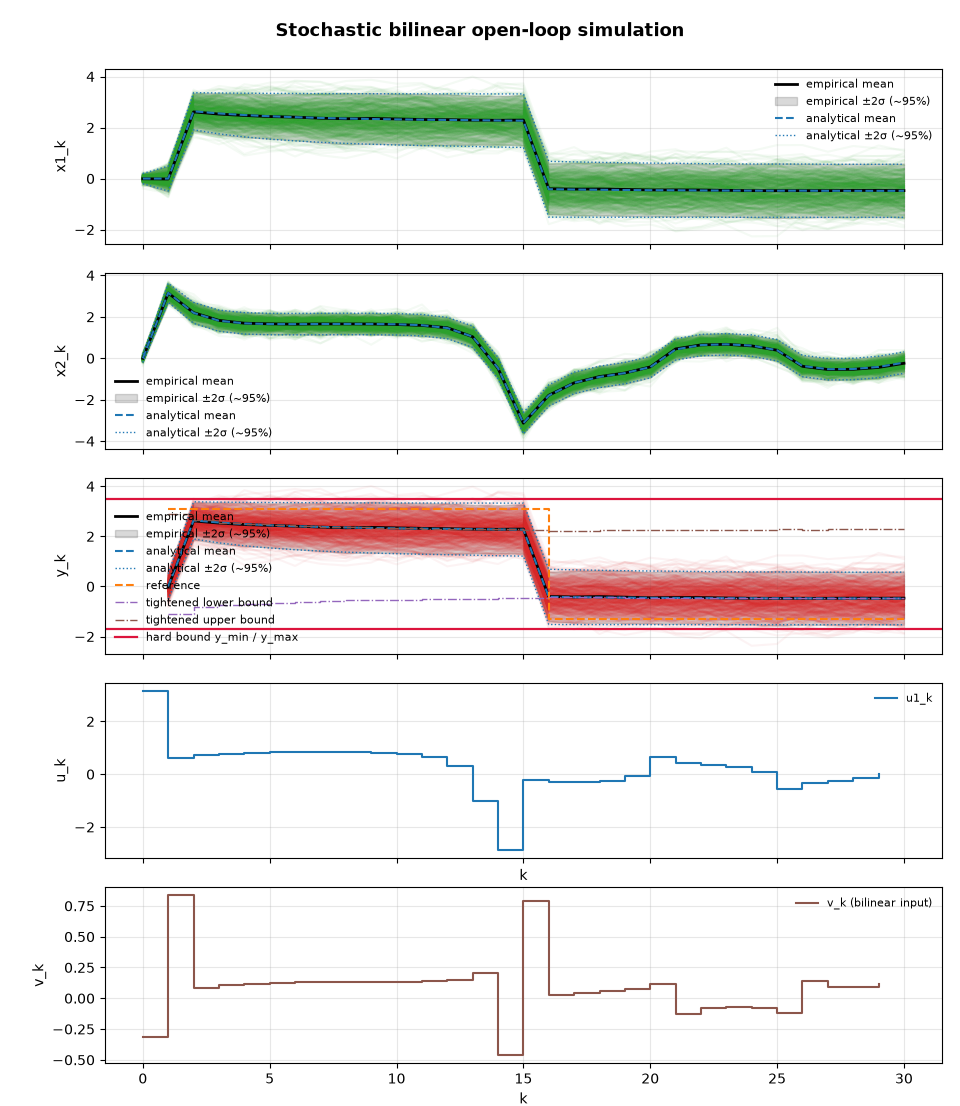
\includegraphics[width=1.0\textwidth]{graphics/Stochastic_Bilinear_Open_Loop_n_500.png}
    \caption{Monte Carlo output trajectories for the stochastic bilinear
    open-loop implementation together with the reference trajectory,
    original constraints, and tight bounds}
    \label{fig:sb_open_loop_outputs}
\end{figure}

\newpage
\section{Closed-Loop Implementation}
\label{sec:sb_closed_loop}

The stochastic bilinear closed-loop controller is implemented using a
receding-horizon Monte Carlo structure similar to the stochastic closed-loop model. But this time for finding optimal U* & V* SLSQP solver used.

\begin{enumerate}
    \item Generate independent initial conditions for all Monte Carlo
    realizations.

    \item At time \(k\), use the current state of each realization as the
    initial condition for its prediction problem.

    \item Construct the current reference trajectory over the prediction
    horizon.

    \item For each candidate \(V\), propagate the bilinear covariance and
    construct the corresponding tight bounds.

    \item Solve the nonlinear constrained optimization problem using SLSQP
    independently for each realization.

    \item Obtain \(U_k^{\ast,(j)}\) and \(V_k^{\ast,(j)}\).

    \item Apply only the first pair
    \[
        u_k^{(j)}=u_{k|k}^{\ast,(j)},
        \qquad
        v_k^{(j)}=v_{k|k}^{\ast,(j)}
    \]

    \item Sample the stochastic disturbances and update the system.

    \item Shift the horizon and repeat the optimization at \(k+1\).
\end{enumerate}

\subsection{Results}
\label{subsec:sb_closed_loop_results}

The closed-loop experiment used the same stochastic bilinear system with the open-loop case.

\begin{figure}[H]
    \centering
    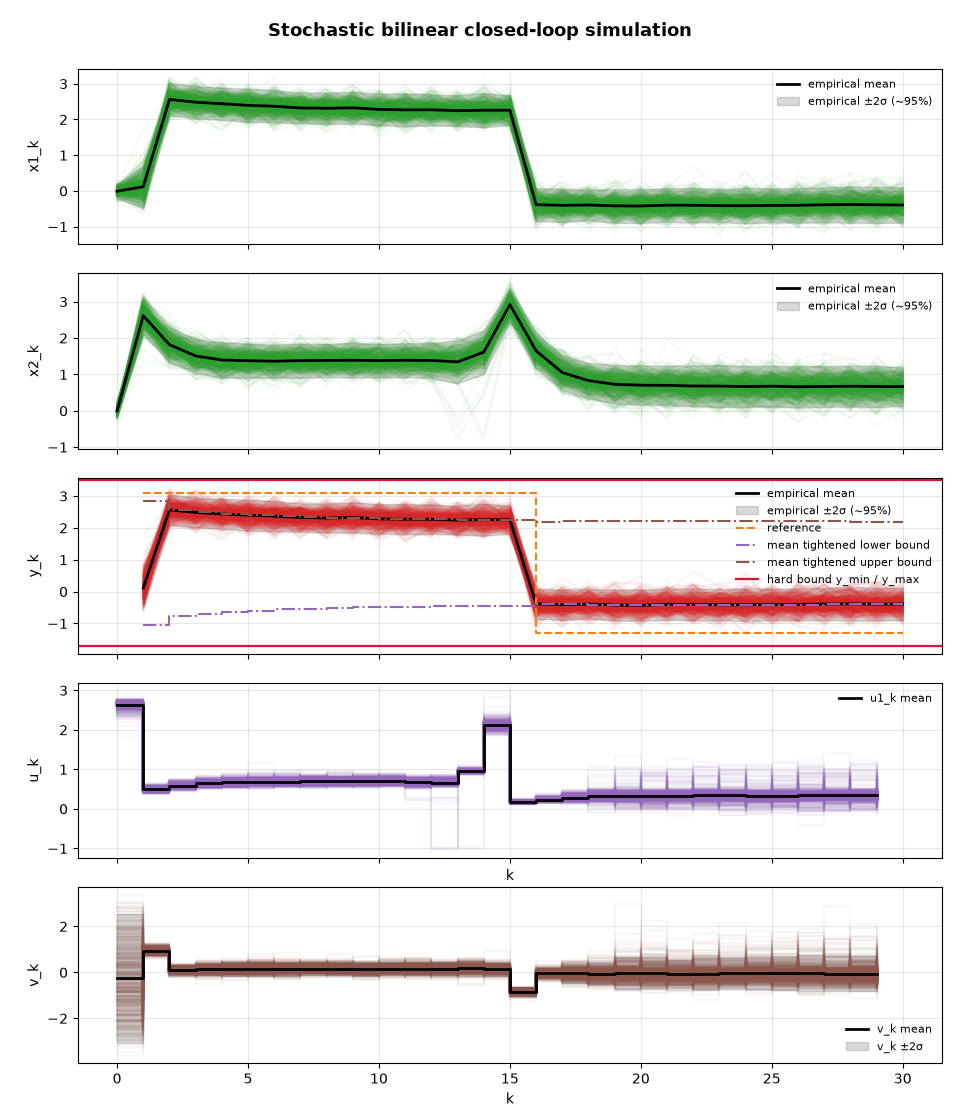
\includegraphics[width=1.0\textwidth]{graphics/Stochastic_Bilinear_Closed_Loop_n_500.png}
    \caption{Monte Carlo output trajectories for the stochastic bilinear
    closed-loop implementation}
    \label{fig:sb_closed_loop_outputs}
\end{figure}
